

\begin{comment}

MAIN REFS


TIELENS, DRAINE, PALLO'S AND OTHERS PAPERS,

DALGARNO\&MCCRAY1972?  GOLDSMITH+12?

FUJIMOTO+19, FUJIMOTO+20

MAYBE SOME OTHER REFS -- FRONTIERS OF COSMO LECTURES?

 SAY THAT WE ARE INTERESTED IN HIGH REDSHIFT GALAXIES -- ZOOM IN (PALLO) SIMULAITONS??


SUMMARY 


 1. INTRO TO HIGH REDSHIFT GALAXIES
 
 2. PHYSICAL CONDITIONS IN THE ISM AND CGM
    (PHASES OVERVIEW)
 
 3. EMISSION IN THE ISM/CGM (COOLING/HEATING)

 4. OBSERVATIONAL PROBES OF HIGH REDSHIFT GALAXIEs (OPTICAL; IR)
 
 5. EXTENDED HALOS PROBES
 
 6. HYPOTHESES FOR THE EXTENDED HALOS FORMATION
 
 7. 
 
 8. 
 
 9. 
 
USEFUL THINGS TO MENTION
 - COOLING/HEATING
 - EQUILIBRIUM CONDITIONS, EINSTEIN COEFFICIENTS ETC
 - PHOTOIONIZATION EQUILIBRIUM
 - ISM/CGM PHYSICAL CONDITIONS
 - EXTENDED HALOS OBSERVATIONS
 
\end{comment}




In the first two chapters of this work, we have laid the foundations of our discussion by presenting a summary of the most important topics in galaxy formation and galactic outflows physics. From now on, we focus on the specific problem our thesis work aims to solve. In this chapter, we present this problem by describing the discovery of extended \CII halos in high redshift galaxies. 

In 2019, Fujimoto et al. \citep{Fujimoto19} reported a "First identification of $10$-kpc Scale \CII $158$ $\mu$m Halos around Star-Forming Galaxies at $z=5-7$". By stacking images of $18$ high-redshift galaxies observed by the ALMA interferometer, these authors were able to unveil the presence of emission of the singly ionized carbon line \CII that was much more extended than the stellar continuum UV emission coming from the corresponding galaxies. 

Gaseous halos had already been identified and studied at low redshift, where a much more detailed analysis of the morphology and physical conditions of the CGM is possible (we introduce these halos in section \ref{sec:general_halos}). However, the presence of diffuse extended \CII emission at high redshift is quite surprising, as it raises a series of challenging theoretical questions that do not find a simple answer in terms of low-redshift halos counterparts. For this reason, after presenting the whole body of observational evidence available to date (section \ref{sec:halo_data}), we elaborate on these questions and their possible answers in section \ref{sec:theory_halos}. We summarize the theoretical studies on \CII emission at high redshift, and we describe the results of zoom cosmological simulations. Finally, we list the most promising solutions that aim to describe the origin of these extended halos. We then focus on the hypothesis that halos at high redshift and galactic winds are strongly connected, describing the arguments in favor of this picture and laying the basis for our outflow model that will be the subject of the next chapter. 





\section{Gaseous halos and the CGM} \label{sec:general_halos}


Gaseous halos are formed by baryons residing in the Circum-Galactic Media of galaxies. As already described in section \ref{sec:feedback}, the CGM is the stage where several processes take place: accreting gas mixes with outflows and galactic fountains. Therefore, it is not uncommon to find halos of diffuse gas in the CGM of star-forming galaxies, resulting from the mutual interaction of these different components (figure \ref{fig:cgm_cartoon}). Several observational techniques can reveal the presence and the properties of these diffuse gas in galaxies' halos \citep[for details, see][]{tumlison}:
\begin{itemize}
    \item Absorption lines in quasars provide information about the objects standing in the QSOs line of sights. Viewing the CGM of a galaxy in absorption against a bright background quasar offers the possibility to explore a wide range of densities - as absorption's measurements have a very high sensitivity - as well as redshifts and luminosities. However, such a technique provides only partial information on the physical conditions of the gas, as it gives only a single, point-like, estimate of the gas surface density. Stacking many different spectra is also a possibility, as it beats down statistical noise, thus enabling measurements of weaker absorbers; however, properties of single systems are averaged out, and physical information such as kinematics and ionization states is thus lost.
    \item Alternatively, a different technique, known as "down-the-barrel" spectroscopy, uses a galaxy’s own starlight as a background source for detecting absorption. This method is commonly used in optical and near-UV lines, to study outflows and/or inflows in low redshift galaxies. The advantage of using down-the-barrel spectroscopy is that it provides key information on the physics of the near-CGM, which is the most interesting region from a physical perspective and it is rarely captured by QSOs absorption studies. An important limitation, however, is that the galactocentric radius of any detected absorption cannot be constrained.
    \item A third possibility is to search directly for light emitted by CGM gas. This emission, scaling as $n^2$, is very challenging to detect. However, this has been done both in nearby galaxies and in higher-redshift ones, probing UV/optical and sub-millimeter wavelengths. Emission maps have the advantage that they can constrain the density profile, morphology, and physical extent of the CGM gas much more in detail than other techniques based on absorption lines. In section \ref{sec:halo_data}, we focus on observations of emission lines in the CGM of high-redshift galaxies.
\end{itemize}
The general picture that emerges from CGM observations hints at a multiphase and dynamically complex structure, hosting a significant fraction of the baryons' budget. The discussion here echoes in many ways the one presented in the context of galactic winds (section \ref{sec:multiphase}): different species probe the presence of many phases characterized by a variety of temperatures and ionization states. A cold and neutral phase ($T\lesssim 10^4\,\mathrm{K}$) coexists with a warmer phase ($T\sim10^{4-6}\,\mathrm{K}$), as well as with hot ionized gas ($T\gtrsim 10^7\,\mathrm{K}$). Evidence for kinematic complexity is then exhibited by the presence of many features in the absorption lines of ions, with different velocities and linewidths. Finally, from the density profiles of CGM gas, the total mass of different phases can be inferred. With this respect, both observations and simulations agree on the fact that the CGM contains a total mass of baryons which is of the same order of magnitude as galaxies' stellar masses. This may contribute to explain why the percentage of baryons residing in stars or in the ISM of galaxies is significantly lower than the one in the IGM (the so-called \textit{missing baryons} problem). An analogous problem concerns the galactic budget of metals (\textit{missing metals}), which can be explained by taking into account the relatively high metallicity of the CGM \citep[e.g.,][]{lehner2018}. 


The analogy we have made with outflows is not accidental. Indeed, one of the major candidates for producing the extended, multiphase CGM is the mixing between the halo gas and galactic winds that continuously takes place as gas flows out of the galaxy \citep{Thompson16,fielding2017impact}. Other scenarios include the presence of cooling inflows driven by thermal instabilities \citep{mccourt2012thermal}, and cool clouds entrained in outflowing/inflowing gas (for more details, see section \ref{sec:outflows_cooling}). Disentangling the relative contributions of these mechanisms is not an easy task, as distinguishing between inflows and outflows is only partially possible. Observations, however, indicate that outflows have a greater covering factor \citep{rubin2014evidence}, suggesting that a large part of the CGM is made of outflows.  


\begin{figure}
	\centering
	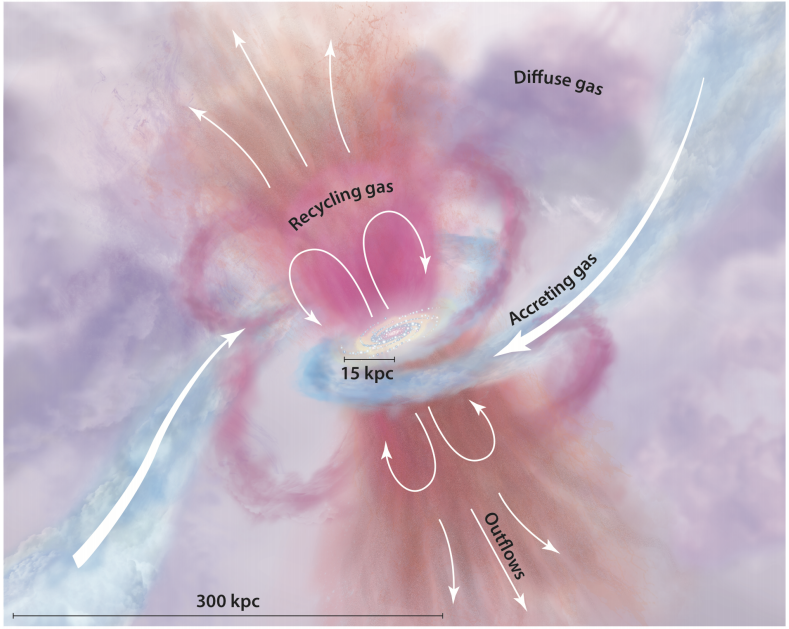
\includegraphics[width=0.6\textwidth]{plots/cgm.PNG}
	\caption{A sketch of the different gas components populating the CGM of a star-forming galaxy. Outflowing/recycling gas is represented in pink and orange, while gas accreting from the IGM has a light blue shade. Tones of purple highlight the presence of diffuse gas in the halo whose source is mixed or unclear. Taken from Tumlinson et al. \citep{tumlison}.
	}
	\label{fig:cgm_cartoon}
    \end{figure}


\section{Observations of halos at high redshift} \label{sec:halo_data}


The discussion presented in the last section provides a partial but reasonable picture of the conditions of the CGM in local and low redshift galaxies. However, in the last few years, new observational capabilities have paved the way to the study of galaxies deep into the Epoch of Reionization ($z\approx6$; see section \ref{sec:first_lights_reionization}). Reionization marks the epoch at which galaxies are still evolving at a fast rate, and start to alter the ionization state of the IGM. Therefore, in this epoch, galaxies are expected to have different morphologies, physical and chemical properties from their local counterparts. For this reason, observations of high redshift galaxies are particularly interesting, as they offer the opportunity to trace back the galactic evolution process, and to shed light on the mechanisms of interaction between galaxies and the pristine medium surrounding them. 

High redshift observations differ from local ones for a variety of reasons. Most importantly, cosmological redshift moves radiation from stars and galaxies in different regions of the electromagnetic spectrum. For redshifts $z\approx 4-7$, UV and optical radiations are shifted to the Near-InfraRed (NIR), while dust emission gets shifted further into the FIR/millimeter wavelengths. Therefore, investigating galaxies in the NIR can offer important information on the light emitted by stars that is not absorbed by dust (i.e., it can probe the so-called \textit{unobscured star formation}). On the other hand, looking at the FIR completes the picture by providing details about the \textit{obscured star formation}. Emission and absorption lines in these two regions of the electromagnetic spectrum can also be used in synergy to study the kinematics, composition, temperature, and density of gas in the ISM/CGM of high-redshift galaxies. This kind of \textit{panchromatic surveys} are routinely used in the local universe, but they have become possible even at higher redshift thanks to the synergy between space telescopes such as the Hubble Space Telescope (HST) and Spitzer and ground telescope such as the Very Large Telescope (VLT), the Atacama Large Millimeter/submillimeter Array (ALMA), and the NOrthern Extended Millimeter Array (NOEMA). 

In particular, the rest-frame UV/optical part of the spectrum has been probed multiple times in the last decade using spectroscopic and imaging surveys \citep[e.g.,][]{oesch2009structure,Shibuya:2015qfa, bouwens2017z, kawamata2018size}. Thanks to these studies, we have now a solid statistical sample that can gauge the evolution of several properties in high redshift galaxies, such as the UV-luminosity function, the size and morphology of the stellar and gaseous components, and the unobscured star formation history. Information from the dust and cold gas emitting in the FIR band, instead, has become available only thanks to the advent of radio-interferometers such as ALMA and NOEMA. In the last few years, these instruments have offered the opportunity to measure continuum (thermal) emission from dust in high redshift galaxies, as well as emission lines from cold ISM gas such as [CII] $158 \,\mu\mathrm{m}$, [O III] $88 \,\mu\mathrm{m}$, and CO from various rotational levels \citep{maiolino2015,capak2015,pentericci2016,knudsen2016b, matthee2017, carniani2018b, Hashimoto2018,gallerani:2018}.

In this work, we focus on spatially-resolved ALMA observations of the \CII line in galaxies at $z\approx 4-7$. The \CII line is created by the fine-structure transition $^2P_{3/2} \rightarrow
\,^2P_{1/2}$ of singly ionised carbon at $\lambda = 158\,\mu\mathrm{m}$. It is one of the brightest lines in the FIR, as it accounts for a significant fraction ($\approx 0.1-1\,\%$) of the total FIR luminosity \citep{gong2012}. Being also very easy to excite, it arises from gas with very different physical properties. We discuss in more detail the theoretical models that describe \CII emission in section \ref{sec:theory_halos}. 

By comparing the spatial extension of \CII with the extension of rest-frame FIR and UV emission, a growing number of works \citep{carniani2018b, Fujimoto19, ginolfi:2019, Fujimoto:2020qzo, herrera2021kiloparsec} have found that the \CII emitting region of galaxies at high-z is significantly more extended than the continuum one. These findings pair with parallel evidence for the presence of extended Ly$\alpha$ line emission at high redshift: as found by e.g., \citet{Wisotzki16}, the effective radius of the Ly$\alpha$ spatial extension on average $\sim 5-15$ times more extended than the central UV continuum. 

As the UV/FIR continuum traces the stellar region - and hence the size of the galaxy - the presence of extended \CII (Ly$\alpha$) emission probes the presence of singly ionized carbon (neutral hydrogen) deep into the CGM of normal star-forming high-z galaxies. In turn, this has profound implications on our understanding of galaxy formation and evolution. Carbon, in particular, plays a key role in this discussion, as it witnesses early gas exchanges between galaxies and their CGM. In fact, while diffuse metal halos at low redshift are compatible with our understanding of feedback and accretion (section \ref{sec:general_halos}), the presence of these extended structures at high-z implies very early contamination of the pristine CGM by the products of stellar nucleosynthesis. Moreover, the ionization state of carbon implied by the presence of massive \CII emission can offer us very important information on the density, temperature, and radiation fields acting on the gas in the surroundings of early galaxies. In the next few paragraphs, we describe in detail the whole body of observations of \CII halos available to date. Theoretical considerations and physical implications of these observations are left for the last section.  






\subsection{First identification}

Early signs of the presence of \CII extended emission at high redshift were found by Cicone et al. \citep{cicone2015} in a massive $z\sim6$ quasar host, using observations taken with the IRAM Plateau de Bure Interferometer (the precursor of NOEMA). By measuring the spatial extent of the \CII line and of the FIR continuum, the authors proved that the former reaches a maximum projected radius of $30$ kpc, while the latter does not exceed $15$ kpc. This extended emission is likely associated with a powerful AGN-driven outflow, as a large part of the gas traced by \CII is at high velocities (i.e., up to $\sim 1400\,\kms$ relative to the systemic velocity). 

The higher sensitivity of ALMA opened up the study of normal star-forming galaxies at the same redshifts. With this respect, a first work by Carniani et al. \citep{carniani2018} used archival ALMA observations to study the properties of \CII emission in normal $z\approx 5-7$ galaxies. They revealed that, in their sample of $29$ galaxies, \CII emission is generally much more extended than the UV emission. However, a similar result needed to be supported by further analyses, as a low signal-to-noise ratio (S/N) and large uncertainties could undermine the reliability of size measurements. 

The work of Fujimoto et al. \citep[][hereafter F19]{Fujimoto19} confirmed the presence of extended \CII halos by stacking several observational data in order to increase the S/N. In the F19 paper, the authors identify in the literature \citep[e.g.,][]{capak2015, maiolino2015, willott2015, pentericci2016, carniani2018} 18 galaxies at $z \approx 5-7$ that met some specific requirements, such as \CII S/N$>5$, no signs of AGN activity or gravitational lensing, SFR$<100\,\msun\mathrm{yr}^{-1}$, \CII line with a Full-Width Half Maximum (FWHM) broader than $80\,\kms$. Using this sample of galaxies, a stacking technique in the $u-v$ visibility plane (i.e. the 2-d transform of the sky brightness plane) is applied to obtain a single emission map with an effective S/N of $21$ and $10$ for the \CII line and the dust continuum respectively. UV continuum HST observations of the same galaxies are stacked as well, and the HST Point Spread Function (PSF) is convolved with a best-fit kernel in order to make it equivalent to the ALMA beam. In this way, a fair comparison between ALMA and HST spatial emission data is possible. 

The left panel of figure \ref{fig:fuji_data} represents the final spatial emission maps of \CII, FIR and UV continuum obtained by following the stacking procedure. On the right panel, the averaged radial profile for these quantities is shown: from this plot, it is easy to conclude that the \CII emission (red) is much more extended than the (rest-frame) FIR and UV ones (green and blue respectively). This result implies that $10$-kpc scale \CII halos surround star-forming galaxies in the early Universe. The existence of these halos is statistically significant at the $9.2\sigma$ level. Exponential fits of the halo profile, as well as of the HST stellar continuum, show that the scale length of the \CII is a factor of $\sim5$ times greater than the continuum's one. This is in agreement with the fact that the typical radius of normal star-forming galaxies at $z\approx 6$ is estimated to be less than $1$ kpc \citep{Shibuya:2015qfa}. Overall, the F19 analysis is the first strong statistical evidence in favor of the existence of extended \CII halos in the CGM of high redshift galaxies.




\begin{figure}
    \centering
    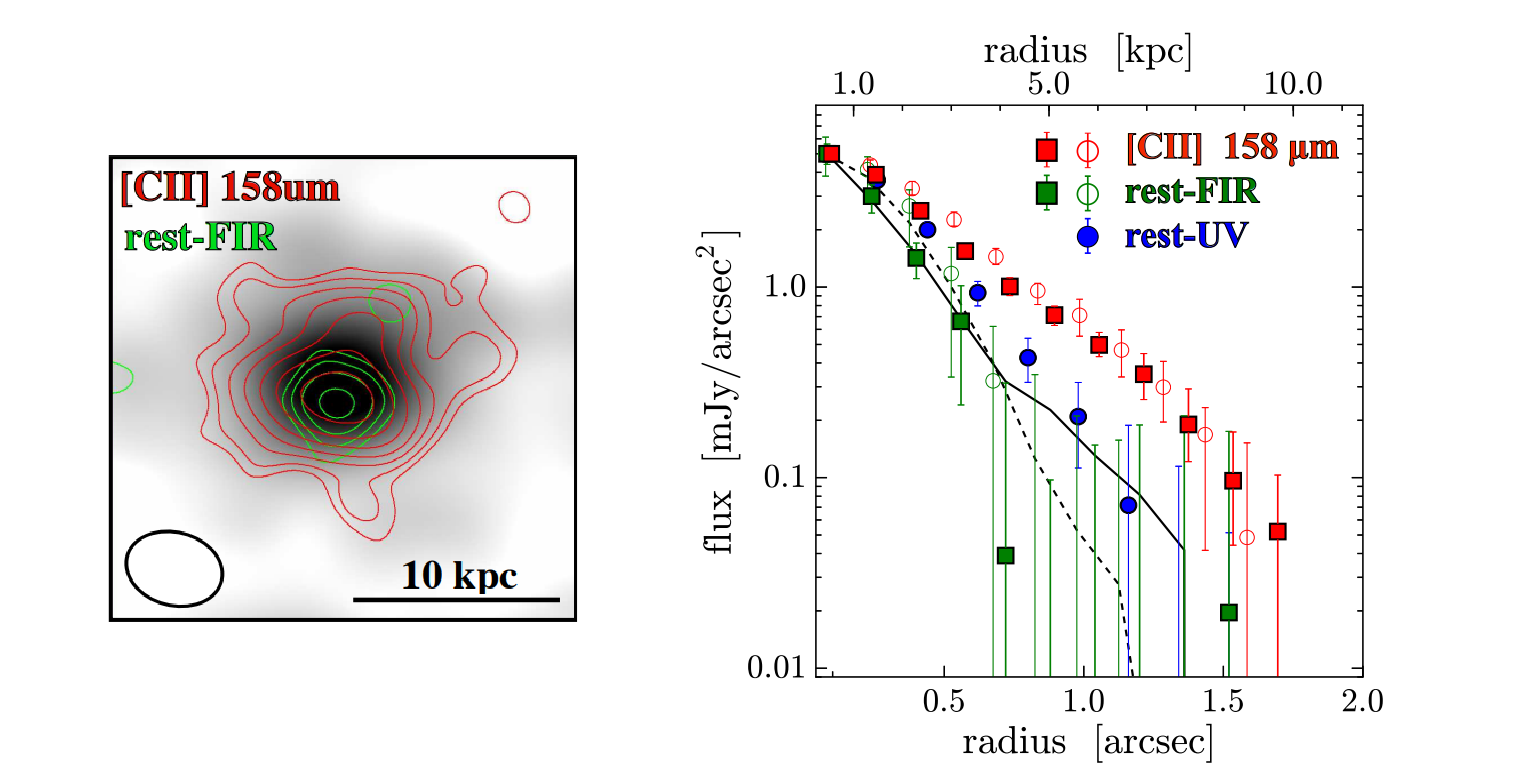
\includegraphics[width=1.0\textwidth]{plots/fuji_data_final.png}
    \caption{\textit{Left:} spatially resolved emission maps taken from F19 \citep{Fujimoto19}. The background image shows the rest-frame UV emission (whose resolution is matched to the ALMA image), while the red and green contours show the \CII line and the (FIR) dust continuum emission respectively. \textit{Right:} averaged radial surface brightness profiles for the F19 \citep{Fujimoto19} sample. The red, green, and blue symbols denote the \CII line, rest-frame FIR, and rest-frame UV continuum emission respectively. Square symbols refer to the whole sample, while circles only include the galaxy for which the HST continuum images are available. The black dashed and solid curves denote the ALMA synthesized beams for these two sub-samples. All radial profiles are normalized to the peak value of the \CII line. 
    }
    \label{fig:fuji_data}
\end{figure}


\begin{figure}
    \centering
    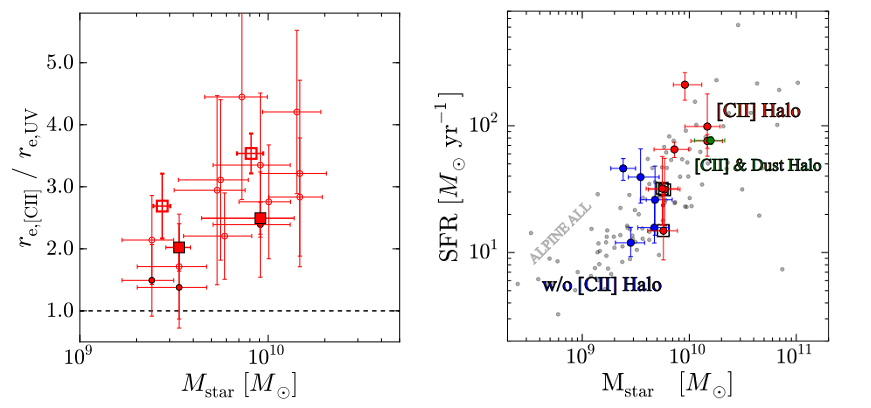
\includegraphics[width=1.0\textwidth]{plots/alpine_effective_radius_final.png}
    \caption{\textit{Left:} ratio of $r_{e,\mathrm{CII}}$ to $r_{e,\mathrm{UV}}$ as a function of the stellar mass $M_\mathrm{star}$ taken from the F20 \citep{Fujimoto:2020qzo} study. The rest-frame UV sizes shown with the open and filled shapes are estimated from the HST F814W and F160 maps, respectively. The circle symbols are the actual data, while the squares represent the median values in bins of $M_\mathrm{star}$. \textit{Right:} scatter in the SFR vs $M_\mathrm{star}$ plane for the sample of ALPINE galaxies (grey dots), taken from F20 \citep{Fujimoto:2020qzo}. Sources labeled as "\CII Halo", "without (w/o) \CII Halos", and "\CII \& Dust Halo" (see text for the definitions) are highlighted using red, blue, and green circles respectively.
    }
    \label{fig:alpine_trends}
\end{figure}


\subsection{Results from the ALMA ALPINE program} \label{sec:alpine}


A few months after the release of the F19 study, the ALPINE ALMA observational data became available \citep{lefevre:2019, faisst:2019, bethermin:2019}. ALPINE (ALMA Large Program to INvestigate C+ at Early Times) is a $69$-hours large ALMA program that started in May 2018 and ended in February 2019. The goal of the program was to explore the gas and dust FIR properties in 118 normal star-forming galaxies at $4.4 < z < 5.9$. For this reason, these galaxies were observed in ALMA Band 7, where the \CII line resides, at a spatial resolution of $\lesssim 1.0''$. The galaxies origin from two fields: the Cosmic Evolution Survey field (COSMOS, \citep{scoville2007field}) and the Extended Chandra Deep Field South (ECDFS, \citep{giacconi_field}). All galaxies are spectroscopically confirmed by either Ly$\alpha$ emission or rest-UV absorption
lines, and they are selected to be brighter than an absolute UV magnitude of $M_{1500} = -20.2$. Observations of the rest-frame UV to optical bands with Keck, VLT, HST, and Spitzer are available, and thus a good amount of ancillary data can complement ALMA observations, giving good estimates of the galaxies' (unobscured) SFR and of their stellar mass. The sample has SFRs between $10\,\msun\mathrm{yr}^{-1}$ and $500\,\msun\mathrm{yr}^{-1}$, and masses in the range $M_* \sim 10^9 - 10^{11} \,\msun$. At the end of the program, \CII line was detected above the $3.5\sigma$ level in $64\%$ of the galaxies, while the FIR continuum detection rate was $19\%$.


\begin{figure}[t]
    \centering
    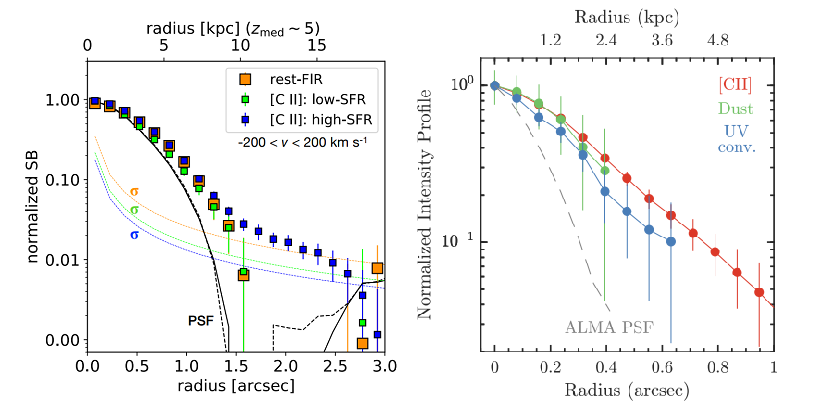
\includegraphics[width=1.0\textwidth]{plots/ginolfi_hc_final.png}
    \caption{\textit{Left:} averaged radial profiles taken from the G19 \citep{ginolfi:2019} stacking analysis; the \CII emission in the $[-200:+200]\,\kms$ range is shown in green squares for the low-SFR sample ($\mathrm{SFR}<25\,\msun\mathrm{yr}^{-1}$), and in blue squares for the high-SFR one ($\mathrm{SFR}>25\,\msun\mathrm{yr}^{-1}$). Orange squares represent the rest-frame FIR continuum, while the solid and dashed black lines represent the ALMA PSF for the whole sample and the continuum-detected sub-sample. \textit{Right}: averaged and normalized radial intensity profiles taken from the HC21 \citep{herrera2021kiloparsec} work. \CII emission (red), rest-frame FIR (dust) continuum (green), and convolved rest-frame UV continuum emission (blue) are shown, as well as the ALMA beam (dashed grey line).
    }
    \label{fig:alpine_data}
\end{figure}

The scientific goals of ALPINE perfectly align with the problem of characterizing the CGM in high redshift galaxies. In particular, spatially resolved emission of the \CII line was obtained for all the galaxies where \CII was detected. These data can provide information on extended halos at a much higher sensitivity than before, allowing a study of halo-hosting galaxies at the individual level, as well as a statistical characterization of their properties. Between 2019 and 2020, two studies presented the results of ALPINE in the context of extended \CII halos. The first one, Ginolfi et al. \citep[][hereafter G19]{ginolfi:2019}, selected a sub-sample of $50$ ALPINE galaxies whose \CII line was detected above a S/N threshold of $5$, and applied stacking procedure both to the \CII line spectra and to the \CII line data-cubes (i.e., the \CII spatial emissions as a function of the wavelength/radial velocity). Their results are particularly interesting, as both of the stackings yield important information on the properties and nature of \CII halos. Stacking the data-cubes and integrating over a $-200\,\kms<v<200\,\kms$ velocity range, they find clear evidence for a \CII structure extending out to the $15\,\mathrm{kpc}$ scale. Considering the spectra, instead, they detect broad-wings features at velocities of few hundreds of $\kms$. These are typical signatures of outflows, as they are created by high radial velocity gas, whereas the central Gaussian component originates from the kinematics of the gas bounded to the central galaxy. Therefore, these findings suggest that both outflows and extended halos are a common feature of star-forming high-z galaxies: this thesis work aims to causally connect these two pieces of evidence by providing a model for an outflow that is able to account for the observed \CII extended emission. 

Another compelling finding from G19 is the dependence of the halo's extension and outflow's features on the star formation rate. By dividing the ALPINE sample into two sub-samples with $\mathrm{SFR}<25\,\msun\mathrm{yr}^{-1}$ and $\mathrm{SFR}>25\,\msun\mathrm{yr}^{-1}$ respectively, they find that the broad-wing feature indicating ongoing outflow activity is much stronger for the high-SFR sub-sample, and that only this latter group of galaxies show the extended halo feature, while the rest of low-SFR galaxies does not show any \CII emission outside the FIR continuum region (figure \ref{fig:alpine_data}). A similar trend is a clear indication that both the observed outflows and the extended \CII structures are created by SF-related processes. We have already described (chapter \ref{chap:outflows}) how outflows can be driven by star formation via the energy and momentum released by SNe and stellar winds. In the next chapter, we argue for a picture where these same SF-driven outflows are responsible for the \CII halos formation.


A second study by Fujimoto et al. \citep[][hereafter F20]{Fujimoto:2020qzo}, then, analyzed the ALPINE sample searching for signatures of \CII halos on the individual level. The authors consider only the ALPINE galaxies that were detected in \CII above $5\sigma$ and that were not classified as mergers by a visual inspection of their morphologies. In this way, only galaxies whose \CII emission is strong and not spuriously created by companions are selected. For every galaxy in this subsample, they use an exponential profile to fit the emission both in \CII and in the rest-frame UV continuum (from HST data). They obtain two effective radii, $r_{e,\mathrm{CII}}$ and $r_{e,\mathrm{UV}}$, representing the extension of the \CII and stellar regions respectively (see the F20 paper \citep{Fujimoto:2020qzo} for details on the fitting procedure). 

Figure \ref{fig:alpine_trends} (left panel) shows the ratio $r_{e,\mathrm{CII}} / r_{e,\mathrm{UV}}$ as a function of the galaxy stellar mass (only measurements that are considered as reliable are shown in the plot). The ratio stays always in the range $2-3$, meaning that the effective size of the \CII region is consistently greater than the UV one. Moreover, there is a clear trend with stellar mass, meaning that the relative size of the \CII extended region is bigger for higher stellar masses. 

In order to investigate this result more carefully, F20 considers the full (averaged) radial profiles for \CII, UV-continuum (from HST), and (when available) FIR-continuum. Matching the resolution of these different quantities -- simply convolving the ALMA profiles with the HST beam and vice-versa --, they obtain emission maps and radial profiles for individual galaxies. Then, they classify these galaxies in three different categories, by looking at the strength of the \CII, FIR, and UV emissions in a "peripheral region" obtained by masking a central area corresponding to the observational beam. A galaxy is defined to host a \CII halo if the statistical significance of the \CII emission in this peripheral region is above the $4\sigma$ level, and, at the same time, the statistical significance of the UV and FIR emissions are below $3\sigma$. Similarly, a galaxy is defined as "without \CII halo" if the statistical significance in this region is below $3\sigma$ for all the \CII, FIR, and UV emissions. 

F20 identifies seven sources (DC$396844$, DC$630594$, DC$683613$, DC$880016$, DC$881725$, VC$5100537582$, and VC$5110377875$) hosting a "CII halo", and six other galaxies not showing signs of extended \CII emission. A third category ("\CII \& Dust halos") is also created for the only object (DC$488399$) showing signs of extended emissions both in \CII and FIR (i.e., dust continuum), but not in UV. Figure \ref{fig:alpine_halos} represent some instances of emission maps and radial profiles for sources hosting a \CII halo, without a \CII halo, and with the \CII \& Dust halo. 

Overall, F20 finds that $\sim 30\%$ of the sources have a \CII halo extending over $15-\mathrm{kpc}$ scales. Note that this number may be even higher, as observational limitations could in principle hamper the identification of fainter halos in the remaining part of the sample. Deeper observations are needed to test whether \CII halos are ubiquitous in normal star-forming galaxies, or form only in a part of them.

Having set a lower bound to the number of galaxies hosting a \CII halo, the authors in F20 can then compare them to the full ALPINE sample, in order to identify some specific features that are correlated with the presence of extended \CII emission. The most significant correlations they find are shown in figure \ref{fig:alpine_trends}, where the distribution of the ALPINE sample in a SFR vs stellar mass scatter plot is displayed. \CII halos (w/o \CII halos) galaxies are highlighted in red (blue) circles. Halo-hosting objects are clearly biased towards higher masses and higher SFR. 

This result is consistent both with the effective radii trend discussed in figure \ref{fig:alpine_trends} and with the result from the ALPINE stacking presented in G19. As already discussed, this could imply a role of star formation in the halos formation process. However, we have to keep in mind that if observational constraints are preventing fainter halos to be observed, then these trends could be simply due to selection biases. On the other hand, there are few sources with similar SFR and $M_\mathrm{star}$ but different halos properties, suggesting that these trends are at least partially valid. 

After completion of the ALPINE program, another observational study by \citet[][hereafter, HC21]{herrera2021kiloparsec} made some important steps forward in the study of \CII emission in normal high-z galaxies. The authors of the study used the ALMA telescope to perform a follow-up observation of the ALPINE system DC$494057$ (also known as HZ$4$) with very high ($\approx 0.3''$) spatial resolution. This system was not part of the F20 "\CII halo" category. However, thanks to the increased resolution of the HC21 study, it has been possible to find strong statistical evidence for the presence of a \CII halo surrounding the HZ$4$ galaxy. The halo extends beyond the star-forming disk and has a radius of $\approx 6$ kpc. Figure \ref{fig:alpine_data} (right panel) shows the averaged radial profiles for the \CII line and the UV/(FIR) emissions. 

Furthermore, the high observational resolution of the HC21 has another key advantage, as it allows to resolve the central regions of the galaxy and to isolate single regions of $\approx 2$ kpc size. Studying the spectral properties of these regions on an individual basis, the authors have found evidence for an outflow that extends from the central regions of the galaxy in the direction of its minor axis. The outflow has a velocity in the range $v\approx 320-420 \kms$ -- consistent with velocities
measured in lower redshift systems -- and a local mass loading factor (section \ref{sec:obs_outflows}) equal to $\eta \approx 3-6$. Overall, these findings seem to suggest that the outflow and the carbon halo are -- at least partially -- causally connected.

\begin{figure}
    \centering
    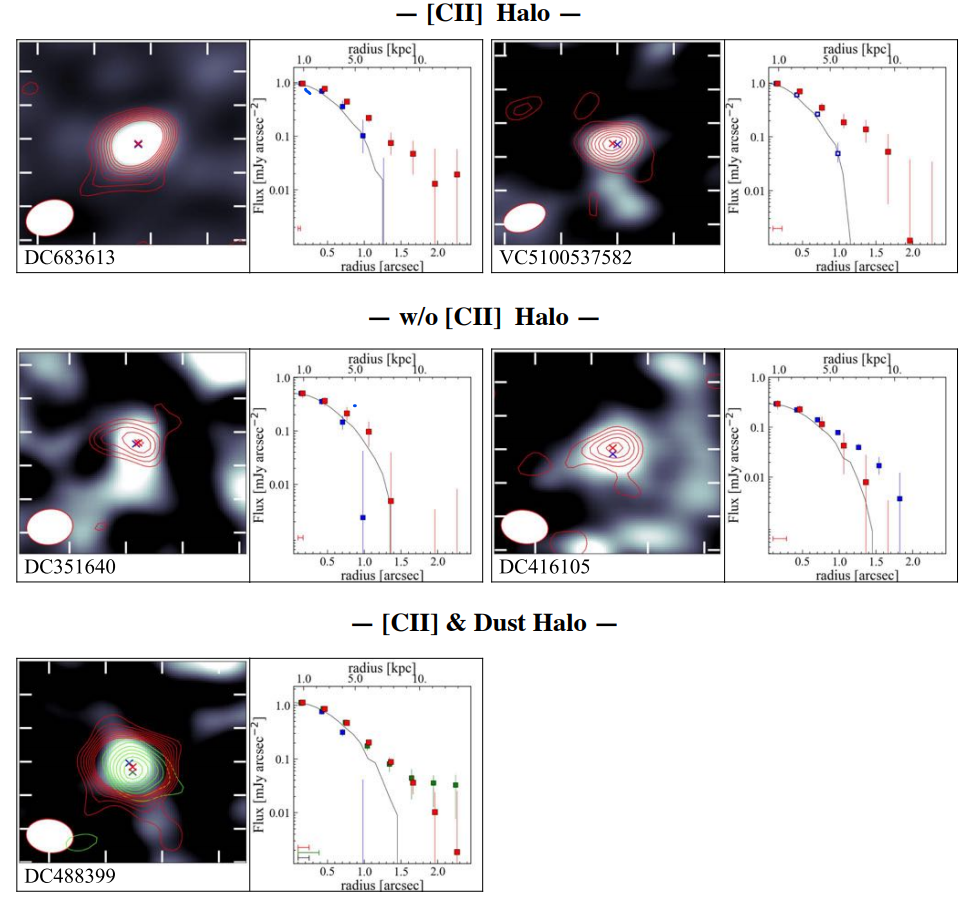
\includegraphics[width=1.0\textwidth]{plots/alpine_halos.png}
    \caption{Instances of ALPINE individual galaxies analyzed in F20 \citep{Fujimoto:2020qzo}. The objects are divided into three categories, as described in the text: "\CII Halo", "without (w/o) \CII Halo", and "\CII \& Dust Halo". On the left panels, the spatial distributions of the \CII line (red), the rest-frame FIR (green, wherever available), and UV continuum (background) are shown. The HST image and ALMA contours are smoothed by the ALMA synthesized beam and the HST PSF, respectively, to match the spatial resolutions between the HST and ALMA maps. Right panels show the averaged radial surface brightness profiles for the \CII line (red squares), the rest-frame FIR (green squares) and UV (blue squares) continuum. The black solid curve shows the ALMA synthesized beam. All profiles are normalized to the \CII one. 
    }
    \label{fig:alpine_halos}
\end{figure}



\section{Insights from theory and simulations} \label{sec:theory_halos}


The body of observational data that has piled up in the last few years poses the existence of \CII halos on very solid ground. For this reason, it is important to interpret the presence of these halos in light of current cosmological models for galaxy formation and evolution. In recent years, several studies have focused on modeling the physical conditions in the ISM and CGM of high-z galaxies, with particular focus on the problem of \CII emission. We briefly review the role that \CII is thought to play in high redshift systems, in order to present the theoretical questions arising from the discovery of \CII halos in the right context. Then, we look at the most promising solutions that may be able to give an answer to the halos problem.

\subsection{[CII] emission in high-z galaxies} \label{sec:CII_models}




The gas in the ISM of galaxies is organized in a variety of phases \citep{tielens2005book}: cold clouds coexist with a hot intercloud medium, as well as with a warm medium, divided in neutral and ionized. These diffuse and low-density components are often accompanied by denser regions, that take different names based on their temperature and composition. \HII regions are made by warm, ionized gas, while (giant) molecular clouds are composed of neutral gas and molecules, and they have a temperature as low as $10\,\mathrm{K}$ (see also sec. \ref{sec:first_lights_reionization}). Photo-dissociation regions (PDR) arise in the outer layers of molecular clouds, where Far-UV radiation (with energy in the range $6-13.6\,\mathrm{eV}$) can penetrate inside because it is not absorbed by neutral hydrogen; as a results, trace species such as carbon and silicon -- whose ionization potential is lower than $13.6\,\mathrm{eV}$ -- become ionized.


The $158\,\mu\mathrm{m}$ \CII emission arises primarily in PDR regions \citep{hollenbach1999}. However, given that its line transition is very easy to excite ($E/k \approx 92\,\mathrm{K}$), it can also trace the diffuse (cold and warm) neutral medium \citep{wolfire2003}, and to a lesser degree even the ionized medium \citep{cormier2012}. The ubiquity of \CII emission makes it one of the major coolants in the ISM, and the brightest line in the FIR window. At high redshifts ($z\gtrsim 4$), this window is conveniently redshifted to sub-millimeter wavelengths, where it can be detected with earth-based telescopes \citep{bethermin:2019}. For this reason, several theoretical studies have focused on determining the relative contribution of different ISM/CGM phases to the \CII luminosity \citep{vallini2015, pallottini2017, pallottini:2019}, as well as the role of gas dynamics \citep{kohandel:2019} and star-formation \citep{vallini2017, ferrara:2019} in the physics governing the \CII emission at high redshifts.

These studies are often base on zoom simulations: a cosmological simulation (sec. \ref{sec:physics_galaxies}) is set up in order to resolve one or more specific systems, reaching a spatial resolution as low as $10\,\mathrm{pc}$ \citep[e.g.][]{pallottini:2019}. With this resolution, the ISM thermochemical non-equilibrium evolution can be followed, including the contribution of chemical, radiative, and mechanical feedback from star formation. \CII emission is usually computed in the post-processing phase, coupling radiative-transfers schemes with physically motivated prescriptions for the ISM. Simulations and other theoretical results agree on the fact that most of the total \CII luminosity arises from the dense PDRs, with little contribution from the diffuse medium \citep[e.g.,][]{vallini2015, pallottini2017}. 


The \CII luminosity profiles predicted by simulations can be compared with the observed extent of \CII emission. Quite surprisingly, even recent and most physically rich zoom simulations fail to reproduce the observed \CII profiles. This is shown in figure \ref{fig:simulations_halos}, by comparing results from F19 \citep{Fujimoto19} with simulations from \citet{pallottini2017b} and \citet{Arata:2019}. These two independent studies agree in predicting a \CII emission that is slightly more extended than the stellar continuum but drops very rapidly at distances considerably smaller than $10\,\mathrm{kpc}$. The resulting profiles are characterized by a value of the surface brightness which, in the external regions, is at least one order of magnitude lower than observed. This mismatch between theory and observation hints either at a non-optimal choice of the parameters governing numerical implementations, or at the presence of some undergoing physical process that has not been completely captured by theoretical models. 


\begin{figure}[t]
    \centering
    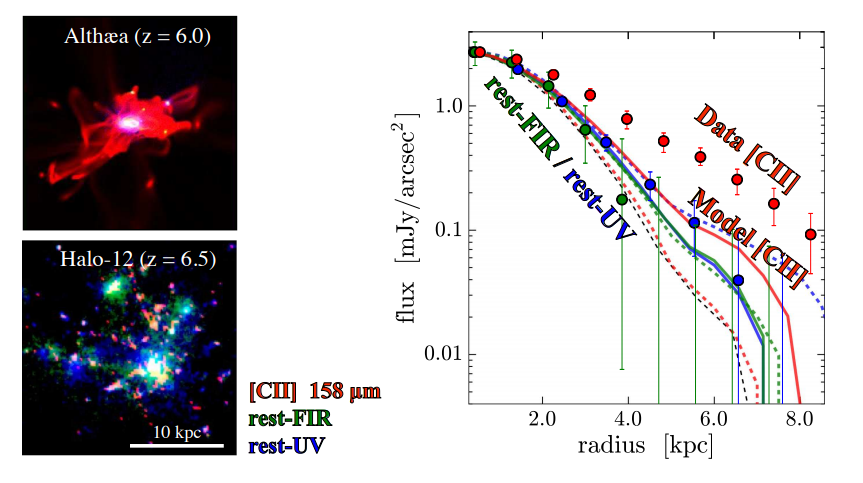
\includegraphics[width=0.85\textwidth]{plots/pallo_sim_halos.PNG}
    \caption{\textit{Left panel}: $4''\times4''$ fake-color image for Althaea (top) and Halo-12 (bottom), obtained from the zoom simulations presented in \citet{pallottini2017} and \citet{arata2019radiative}, respectively (red: \CII line; green: rest-frame FIR continuum; blue: rest-frame UV continuum). \textit{Right panel}: radial averaged surface brightness profiles for the \CII line (red curve), rest-frame FIR (green curve), and UV (blue curve) continuum emission, obtained by stacking the profiles from zoom simulations. The solid and dashed color lines present the Althaea and Halo-12 results, respectively. The black dashed curve denotes the ALMA synthesized beam. Circles indicate the measured profiles obtained by the F19 stacking \citep{Fujimoto19} (same as figure \ref{fig:fuji_data}, left panel). Figure taken from F19 \citep{Fujimoto19}.
    }
    \label{fig:simulations_halos}
\end{figure}

\subsection{Open questions and candidate solutions}

\begin{figure}
    \centering
    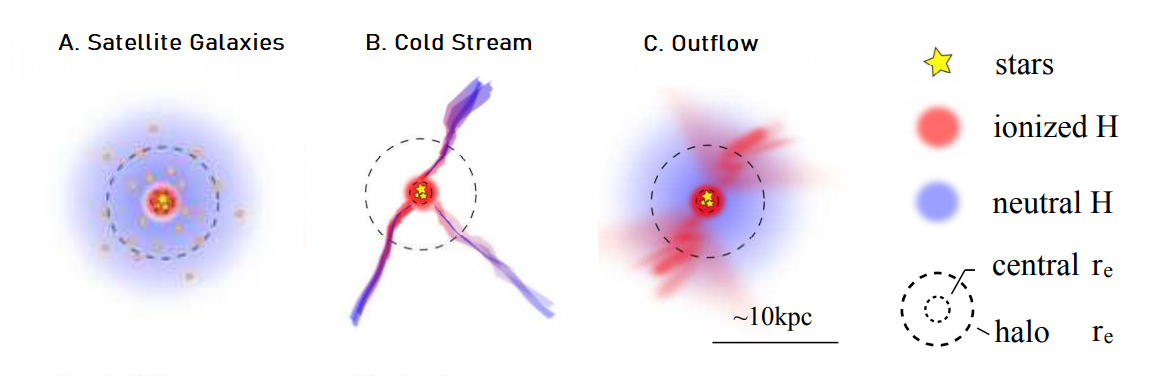
\includegraphics[width=1.0\textwidth]{plots/solutions_final.png}
    \caption{Sketches of three possible scenarios for the physical origin of the \CII halos: A) satellite galaxies; B) cold streams; and C) outflows. Neutral (ionized) hydrogen in the ISM and CGM is shown in blue (red), while yellow stars represent the star-forming regions. The inner and outer dashed circle denote the effective radii ($r_e$) of the central and \CII halo components, respectively. Figure adapted from F19 \citep{Fujimoto19}.
    }
    \label{fig:solutions_halos}
\end{figure}

From the discussion presented in the last paragraphs, it is clear that explaining the origin of extended halos at high redshift, as well as investigating their evolution over cosmic time, is a formidable problem in galaxy evolution. In particular, a number of questions need to be addressed by any theoretical arguments aiming to solve the puzzle of \CII halos:
\begin{itemize}
    \item First of all, the presence of carbon (and presumably other heavy elements) far away from the center of the galaxy questions current models of galaxy evolution. In fact, at high redshift, the gas composing the CGM/IGM of galaxies is expected to have a very low metallicity, since metals are formed only by stars in the central regions of the galaxies. The presence of significant carbon emission implies that carbon has had to be either transported away from the galaxy or created by hidden star-formation activity in the external galactic environment. By what means, then, has carbon been transported to these large distances from the galactic center? How is it present in such a massive amount in the CGM of galaxies?
    \item Even if enough carbon is present in the halo region of galaxies, there is no guarantee that \CII emission matches the observed one. That is because, as we have summarized in section \ref{sec:CII_models} and as we will elaborate on in section \ref{sec:cooling}, the \CII line is created only by specific conditions of gas temperature and density. Which thermodynamics conditions, then, are present in the CGM of halos' hosting galaxies?
    \item A third interesting question involves the ionization state of the gas: a bright \CII line implies that carbon remains singly ionized even in the very low-density region of the CGM. This fact seems to be incompatible with the presence of an ionizing cosmic UV background produced by other galaxies and quasars: low-density, unshielded environments such as the Ly$\alpha$ forest \citep[e.g.,][]{Dodorico13} usually host carbon in higher ionization states. Which is the ionization state of carbon in the halo? Is \CIIion dominant or is it a trace species in a \CIIIion -- dominated environment?
    \item At high redshifts, many physical processes come at play in determining the final luminosity of the \CII line \citep[e.g.,][]{gong2012, vallini2015, kohandel:2019}. For instance, theoretical arguments predict that high-z CMB photons suppress the \CII luminosity considerably (see section \ref{sec:CMB_suppression}). How can this be reconciled with observations? 
    \item Finally, what do \CII halos teach us about high-z systems? What properties of primordial galaxies can be inferred by the presence of extended \CII emission? 
\end{itemize} 

Different scenarios have been proposed so far to account for the extended \CII emission feature. The most complete and convincing ones are: (A) the presence of satellite galaxies; (B) cold streams inflowing inside the galaxy from the IGM; (C) galactic outflow activity. These three hypotheses are sketched in figure \ref{fig:solutions_halos}.

In principle, the emission from a population of faint dwarf galaxy satellites is a good candidate for solving the problem. Faint galaxies cannot be resolved by observations, as they have a surface brightness that is too low to be seen against noise. However, they could give a non-negligible contribution to the observed \CII luminosity. According to this hypothesis, carbon would not be transported from the central galaxy to the outer CGM. Instead, it would be created directly in the halo region by hidden (i.e., not visible in observations) SF activity. This \CII emission would simply arise from the PDR/warm neutral regions of the ISM in satellite galaxies. Indeed, faint satellite galaxies are present in appreciable numbers in zoom simulations \citep[e.g.,][]{pallottini:2019}. However, they are not able to provide a sufficient luminosity to account for the observed \CII emission. In addition, this hypothesis suffers from some theoretical and observational inconsistencies. First of all, from the mass-metallicity relation for galaxies \citep{mannucci:2012}, it is expected for these dwarf satellites to have very low metallicities. This is problematic, as \CII emissivity is directly proportional to the abundance of carbon in the gas (section \ref{sec:cooling}). Furthermore, from figure \ref{fig:fuji_data} we see that the ratio between the \CII and the stellar continuum surface brightnesses gets significantly higher in the galactic outskirts. This is hard to explain with a model where \CII emission arises only in SF regions. Indeed, F19 \citep{Fujimoto19} derive the radial ratio of the \CII luminosity to the total SFR, and find that, in the outer halo area, the ratio becomes much higher than the typical ratio for faint, low-mass galaxies \citep{diaz_santos}. This body of observational and theoretical evidence indicates that satellite galaxies are difficult to be the main cause of \CII halos.


Cold accreting gas streams are considered to be one of the most important ways in which galaxies increase their gas content. We have described the different mechanisms of accretion and the properties of cold streams in section \ref{sec:accretion}. These streams are an interesting candidate because they host a cold/warm dense environment that is suitable to \CIIion. However, the same problem as before applies here: cold streams transport gas coming directly from the IGM, and at high-redshifts, this gas has a very low metallicity because it has yet to be contaminated by heavy elements created inside galaxies. Simulations \citep[e.g.,][]{pallottini2014} find $Z\lesssim 10^{-3}$ at $z=4-6$. Such a low amount of metals is incompatible with the presence of massive \CII emission, and thus this hypothesis lacks support from theoretical arguments.


According to the \textit{outflow hypothesis}, instead, halos represent an incarnation of outflows driven by powerful episodes of star formation and/or active galactic nuclei (AGN) activity occurring in high-z galaxies. As described in section \ref{sec:feedback} and in chapter \ref{chap:outflows}, AGN and starburst-driven outflows are expected to play a major role in galaxy formation, and their ubiquitous presence has been widely recognized. They dominate the CGM gas budget, and, coming directly from the central galactic regions, they can have relatively high carbon contents (see section \ref{sec:outflow_model}). Therefore, if suitable thermodynamic conditions are present in the outflowing gas, a sufficient amount of \CII emission could arise, originating the \CII halos identified by observations. With this respect, many observational hints point towards outflows as a viable solution to the \CII halos dilemma: as already described in section \ref{sec:halo_data}, signs of outflows were identified and linked to \CII extended emission by \citet{cicone2015}, \citet{gallerani:2018}, \citet{ginolfi:2019}, \citet{Fujimoto:2020qzo}, and \citet{herrera2021kiloparsec}. These pieces of evidence are encouraging, and they point at outflows as the most likely explanation for the problem of extended halos formation. 

